\documentclass[a4paper]{report}
% Shared preamble for the English probability and statistics documents.
% Based on the original course preamble. Compile with pdfLaTeX.
\usepackage[top=1.5cm,bottom=2cm,left=2cm,right=2cm]{geometry}
\usepackage[T1]{fontenc}
\usepackage{lmodern}
\usepackage[utf8]{inputenc}
\usepackage[english]{babel}

\usepackage{amsmath}
\usepackage{amssymb}
\usepackage{amsthm}
\usepackage{mathrsfs}
\usepackage{mathtools}
\usepackage{etoolbox}
\usepackage{tikz}
\usetikzlibrary{shapes.multipart,arrows.meta}
\usepackage{xcolor}
\usepackage{enumerate}
\usepackage[shortlabels]{enumitem}
\usepackage{hyperref}
\usepackage{version}
\usepackage{bbold}
\usepackage{fontawesome5}
\usepackage{fancyhdr}
\lfoot{}
\usepackage{natbib}
\usepackage{graphicx}
\usepackage{pdfpages}
\usepackage{authblk}
    
\usepackage{blindtext}
\usepackage{multicol}
\usepackage{collcell}
\usepackage{wrapfig}
\usepackage{blkarray}
\usepackage{cancel}
\usepackage{appendix}
\usepackage{float}
\makeatletter
\input{tex/assets/slashbox.sty}
\makeatother
\hypersetup{unicode,colorlinks,citecolor=red,filecolor=black,
  linkcolor=red,urlcolor=cyan}
\setlength{\columnsep}{1cm}
\pagenumbering{gobble}

\def\numtext#1{%
  \ifcase#1\or one\or two\or three\or four\or five\or six\or seven\or eight\or nine\or ten\or
  eleven\or twelve\or thirteen\or fourteen\or fifteen\or sixteen\or seventeen\or eighteen\or nineteen\or twenty\or Lots\fi}

\newcommand{\Byte}[1]{%
  \def\nodecontents{}%
  \foreach[count=\l] \k in {#1} {\xappto{\nodecontents}{\noexpand\nodepart{\numtext{\l}}\k}}%
  \node[rectangle split,rectangle split parts=8,rectangle split horizontal,draw] at (2,2){\nodecontents};}

\newcommand{\D}{{\mathrm{d}}}
\newcommand{\cE}{{\mathcal{E}}}
\newcommand{\cG}{{\mathcal{G}}}
\newcommand{\cX}{{\mathcal{X}}}
\newcommand{\cY}{{\mathcal{Y}}}
\newcommand{\cB}{{\mathcal{B}}}
\newcommand{\cF}{{\mathcal{F}}}
\newcommand{\cO}{{\mathcal{O}}}
\newcommand{\cS}{{\mathcal{S}}}
\newcommand{\cT}{{\mathcal{T}}}
\newcommand{\given}{\, \big| \,}
\newcommand{\cL}{{\mathscr{L}}}
\newcommand{\cD}{{\mathcal{D}}}
\newcommand{\cA}{{\mathscr{A}}}
\newcommand{\cP}{{\mathscr{P}}}
\newcommand{\cR}{{\mathscr{R}}}
\newcommand{\A}{{\mathcal A}}
\newcommand{\one}{\mathbb{1}}
\newcommand{\mathbbm}[1]{\mathbb{#1}}

\providecommand{\C}{}
\renewcommand{\C}{\mathbb C}
\newcommand{\R}{\mathbb R}
\newcommand{\Q}{\mathbb Q}
\newcommand{\N}{\mathbb N}
\newcommand{\T}{\mathbb T}
\newcommand{\F}{\mathbb F}
\renewcommand{\P}{\mathbb P}
\newcommand{\Z}{\mathbb Z}
\newcommand{\E}{\mathbb {E}}
\newcommand{\Pbb}[1]{\P\left( #1\right)}
\newcommand{\Ebb}[1]{\E\left[ #1\right]}

\newcommand{\lb}{\left (}
\newcommand{\rb}{\right )}
\newcommand{\lbb}{\left [}
\newcommand{\rbb}{\right ]}
\newcommand{\labs}{\left |}
\newcommand{\rabs}{\right |}
\newcommand{\lbrb}[1]{\lb #1 \rb}
\newcommand{\lbbrbb}[1]{\lbb#1\rbb}
\newcommand{\labsrabs}[1]{\labs#1\rabs}
\newcommand{\lbbrb}[1]{\lbb#1\rb}
\newcommand{\lbrbb}[1]{\lb#1\rbb}
\newcommand{\langlerangle}[1]{\langle#1\rangle}
\newcommand{\lbcurly}{\{}
\newcommand{\rbcurly}{\}}
\newcommand{\curly}[1]{\lbcurly#1\rbcurly}
\newcommand{\abs}{\labsrabs}
\newcommand{\ind}[1]{1_{#1}}
\newcommand{\indep}{\perp \!\!\! \perp}
\renewcommand{\d}{\, \mathrm{d}}

\newtheorem{theorem}{Theorem}
\newtheorem{problemCnt}{Lemma}
\theoremstyle{definition}
\newtheorem{problem}[problemCnt]{Problem}
\newtheorem{problembook}[problemCnt]{\faBook \,  Problem}
\newtheorem{problempencil}[problemCnt]{\faPencil* \,  Problem}
\newtheorem{problemstar}[problemCnt]{\faStar\,  Problem}
\newtheorem{problemstarpencil}[problemCnt]{\faStar \, \faPencil* \,   Problem}
\newtheorem{probleminteresting}[problemCnt]{\faSmile[regular] \,   Problem}
\newtheorem{solution}{Solution}

\newcommand{\fwcell}[1]{\makebox[\arraystretch\normalbaselineskip]{$#1$}}
\newenvironment{enumeratei}{\begin{enumerate}[(i)]}{\end{enumerate}}
\newenvironment{enumeratea}{\begin{enumerate}[(a)]}{\end{enumerate}}
\newenvironment{enumeraten}{\begin{enumerate}[\upshape 1.]}{\end{enumerate}}

% Compatibility helpers needed by a few files in the combined archive.
\AtBeginDocument{\noindent{\footnotesize English translation prepared with ChatGPT (OpenAI, GPT-6), 26 October 2026, for translation of the Bulgarian text into English and LaTeX formatting.
The Bulgarian originals remain the reference; translation may contain errors.}\par\smallskip}
\newcommand{\MissingGraphic}[1]{%
  \begin{center}\fbox{\parbox{0.82\linewidth}{\centering Missing source image: \texttt{#1}}}\end{center}}



\setlength{\emergencystretch}{3em}
\allowdisplaybreaks
\begin{document}


\noindent Probability and Statistics, 21.01.2023 \hfill Test 2

\hrulefill

\begin{it}
The exact grading formula depends on the results. As an approximation, use 2 plus the points earned. Time allowed: 3 hours. Good luck.

Throughout, we work on a probability space $(\Omega, \cF, \P)$.

Recall that
the recurrence
$a_n = A a_{n-1} + B$
has solution
$a_n = C_1 A^n + C_2$,
where the constants
$C_1,C_2$ are determined
by the initial conditions.

\end{it}

\begin{problem}
Let $X,Y$ have joint density $f_{X,Y}(x,y)=cx^2+1$ for $x,y\geq0$, $x+2y\leq1$, and zero elsewhere, where $c$ is
a constant. Find:

\begin{enumerate}

    \item (0.5 points) $c$, the density of $X$ and the expectation of $Y$;
\item (0.25 points) $\E(Y|X=1/2)$;
\item (0.25 points) the density of $Z=X+2Y$.

\end{enumerate}

\end{problem}

\begin{problem} A shop is open from 10:00 to 18:00. Model the times between successive arrivals of customers under 30 as independent exponential
variables with mean 5 minutes, and the times between successive customers over 30 as independent exponential variables with mean 10 minutes.

\begin{enumerate}
    \item (0.5 points) What is the probability that at least 100 customers under 30 visit in one day?
    \item (0.25 points) Find the distribution of the waiting time for the first customer of the day.
    \item (0.25 points)
    You may assume that the times between successive customers are independent and have the distribution in part 2\footnote{Bonus**: Prove this.}. What is the probability that at least 150 people visit in one day?
\end{enumerate}

\end{problem}

\begin{problem} A point starts at the origin. At each step it chooses one
of the coordinate directions uniformly and moves one unit. The figure below shows a sample path of 10 steps.

\begin{center}

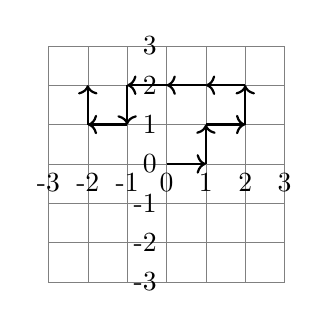
\begin{tikzpicture}[scale=0.5]
\draw[step=1cm,gray,very thin] (-3,-3) grid (3,3);
\foreach \x in {-3,-2,...,3} { \node[anchor=north] at (\x,0) {\x}; }
\foreach \y in {-3,-2,...,3} { \node[anchor=east] at (0,\y) {\y}; }

\coordinate (start) at (0,0);
\coordinate (step1) at (1,0);
\coordinate (step2) at (1,1);
\coordinate (step3) at (2,1);
\coordinate (step4) at (2,2);
\coordinate (step5) at (1,2);
\coordinate (step6) at (0,2);
\coordinate (step7) at (-1,2);
\coordinate (step8) at (-1,1);
\coordinate (step9) at (-2,1);
\coordinate (step10) at (-2,2);

\draw[->, thick] (start) -- (step1);
\draw[->, thick] (step1) -- (step2);
\draw[->, thick] (step2) -- (step3);
\draw[->, thick] (step3) -- (step4);
\draw[->, thick] (step4) -- (step5);
\draw[->, thick] (step5) -- (step6);
\draw[->, thick] (step6) -- (step7);
\draw[->, thick] (step7) -- (step8);
\draw[->, thick] (step8) -- (step9);
\draw[->, thick] (step9) -- (step10);
\end{tikzpicture}

\end{center}

\begin{enumerate}
\item (0.5 points)
What is the probability that its $x$-coordinate exceeds 10 after 1000 steps?
\item (0.5 points) Find the expectation\footnote{Bonus***: And the variance!} of the squared distance from the origin after
$100$ steps.

 \end{enumerate}
\end{problem}



\begin{problem}
Let $X_0\sim Exp(1)$ and $X_n=2X_{n-1}+\epsilon_n$ for $n\in\N$, where the $\epsilon_n$ are independent $N(0,1)$ random variables.
\begin{enumerate}

\item (0.25 points) Find $\E X_n$ and $D X_n$.
\item (0.25 points) Let $S_{n,1}=\sum_{i=1}^n(X_i-2X_{i-1})^2$ and
$S_{n,2}=\sum_{i=1}^n|X_i-2X_{i-1}|$. Find $\E S_{n,1}$ and $\E S_{n,2}$.

\item (0.5 points) Can you answer parts 1 and 2 when $\epsilon_i\sim N(1,2)$?








 \end{enumerate}

\end{problem}































































\end{document}
